\documentclass[11pt,a4paper]{article}
\usepackage{geometry}
\geometry{a4paper, margin=1in}
\usepackage{graphicx}
\usepackage{tikz}
\usepackage{xcolor}
\usepackage{titlesec}
\usepackage{hyperref}

% Couleurs personnalisées
\definecolor{ugablue}{RGB}{0,61,165}
\definecolor{ugagreen}{RGB}{128,189,0}
\definecolor{ugared}{RGB}{206,17,38}
\definecolor{ugayellow}{RGB}{255,200,47}
\definecolor{ugapurple}{RGB}{106,0,155}

% Style des sections
\titleformat{\section}
{\normalfont\Large\bfseries\color{ugablue}}
{\thesection}{1em}{}

\titleformat{\subsection}
{\normalfont\large\bfseries\color{ugablue}}
{\thesubsection}{1em}{}

\titleformat{\subsubsection}
{\normalfont\normalsize\bfseries\color{ugablue}}
{\thesubsubsection}{1em}{}

% En-tête et pied de page
\usepackage{fancyhdr}
\pagestyle{fancy}
\fancyhf{}
\fancyhead[L]{
\includegraphics[height=0.8cm]{uga.png}}
\fancyhead[R]{\textcolor{ugablue}{Assistant pour les preuves de transformations de graphes (style Hoare)}}
\fancyfoot[C]{\thepage}

% Ajuster la hauteur de l'en-tête
\setlength{\headheight}{26.84232pt}

% Page de titre
\begin{document}

\begin{titlepage}
    \begin{tikzpicture}[overlay, remember picture]
        % Triangle bleu
        \fill[ugablue] (0,0) -- (3,4) -- (6,0) -- cycle;
        % Triangle vert
        \fill[ugagreen] (2,0) -- (5,4) -- (8,0) -- cycle;
        % Triangle rouge
        \fill[ugared] (4,0) -- (7,4) -- (10,0) -- cycle;
        % Triangle jaune
        \fill[ugayellow] (6,0) -- (9,4) -- (12,0) -- cycle;
        % Triangle violet
        \fill[ugapurple] (8,0) -- (11,4) -- (14,0) -- cycle;
    \end{tikzpicture}
    
    \vspace*{6cm}
    
    \begin{center}
        {\Huge\bfseries \textcolor{ugablue}{Assistant pour les preuves de transformations de graphes (style Hoare)}}
        
        \vspace{1cm}
        
        {\LARGE \textcolor{ugablue}{En cours de développement - Version 3}}
        
        \vspace{2cm}
        
        {\Large \textcolor{ugablue}{Sébastien Andres - Thomas Ceresa - Rachid Echahed}}
        
        \vfill
        
        
\includegraphics[width=0.4\textwidth]{uga.png}
    \end{center}
    
\end{titlepage}

\tableofcontents

\newpage

\section{Introduction}
Ce guide d'utilisation vous fournira des instructions détaillées sur l'utilisation de notre application. L'application est en cours de développement et ceci est la version 3. Contact: \texttt{thomas.ceresa@etu.univ-lyon1.fr}

\section{Prérequis}
Interpréteur Python3 : cf. \url{https://www.python.org/}
\subsection{Installation Linux (Ubuntu-Debian)}
  \begin{itemize}
	\item pip3, outil d’installation des modules de Python (si besoin) : \texttt{sudo apt-get install python3-pip}
	\item ply, module pour l’analyse lexicale et syntaxique : \texttt{sudo pip3 install ply}
	\item z3 solver, module pour vérifier les formules : \texttt{sudo pip3 install z3-solver}
	\item Flask, mini-framework web : \texttt{sudo pip3 install flask}
  \end{itemize}
\subsection{Installation Windows}
Normalement, pip est installé avec Python3, sinon suivre ces indications : \url{https://pip.pypa.io/en/stable/installation/}\\

Dans un terminal : 
 \begin{itemize}
 \item \texttt{pip install ply}

\item \texttt{pip install z3-solver}

\item \texttt{pip install flask}
  \end{itemize}

\section{Exécution}
Le fichier à exécuter est \texttt{mainFlask.py}. Il se trouve dans le répertoire \texttt{Interface}.\\
Utiliser l'IDE de votre convenance ; ou en console : \texttt{python3 mainFlask.py} (\texttt{py mainFlask.py} sous Windows)\\
Lorsque le programme est exécuté, un serveur web est installé sur la boucle locale avec le numéro de port 5000.\\
Écrire l’adresse \url{http://localhost:5000} dans la barre d’adresse d’un navigateur pour utiliser le logiciel.

\section{Utilisation}
L'application permet de saisir des preuves, de les enregistrer et de les lire. Dès l'écran d'accueil, choisissez de lire un fichier ou de le saisir manuellement.
\begin{figure}[htbp]
  \centering
  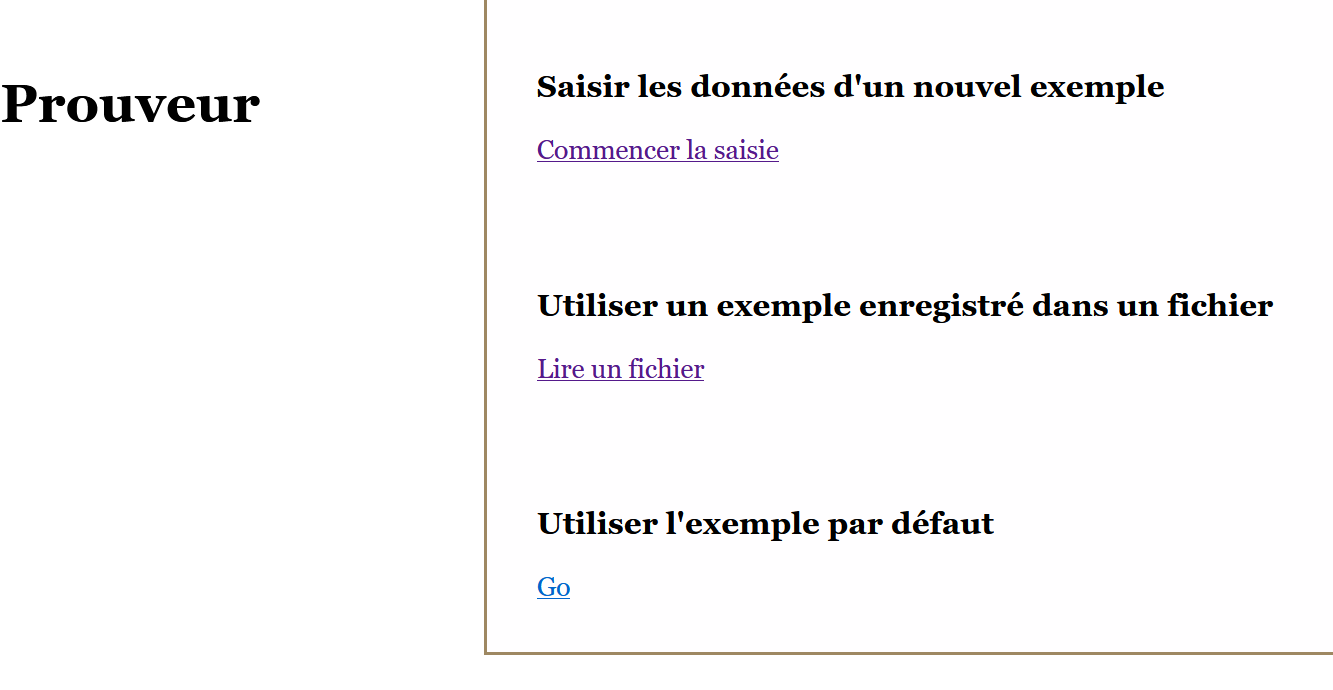
\includegraphics[width=0.6\textwidth]{screen4.png}
  \caption{Écran d'accueil}
  \label{fig:mon_image}
\end{figure}
\subsection{Vue d'ensemble}
Les preuves sont présentées comme suit:
\begin{figure}[htbp]
  \centering
  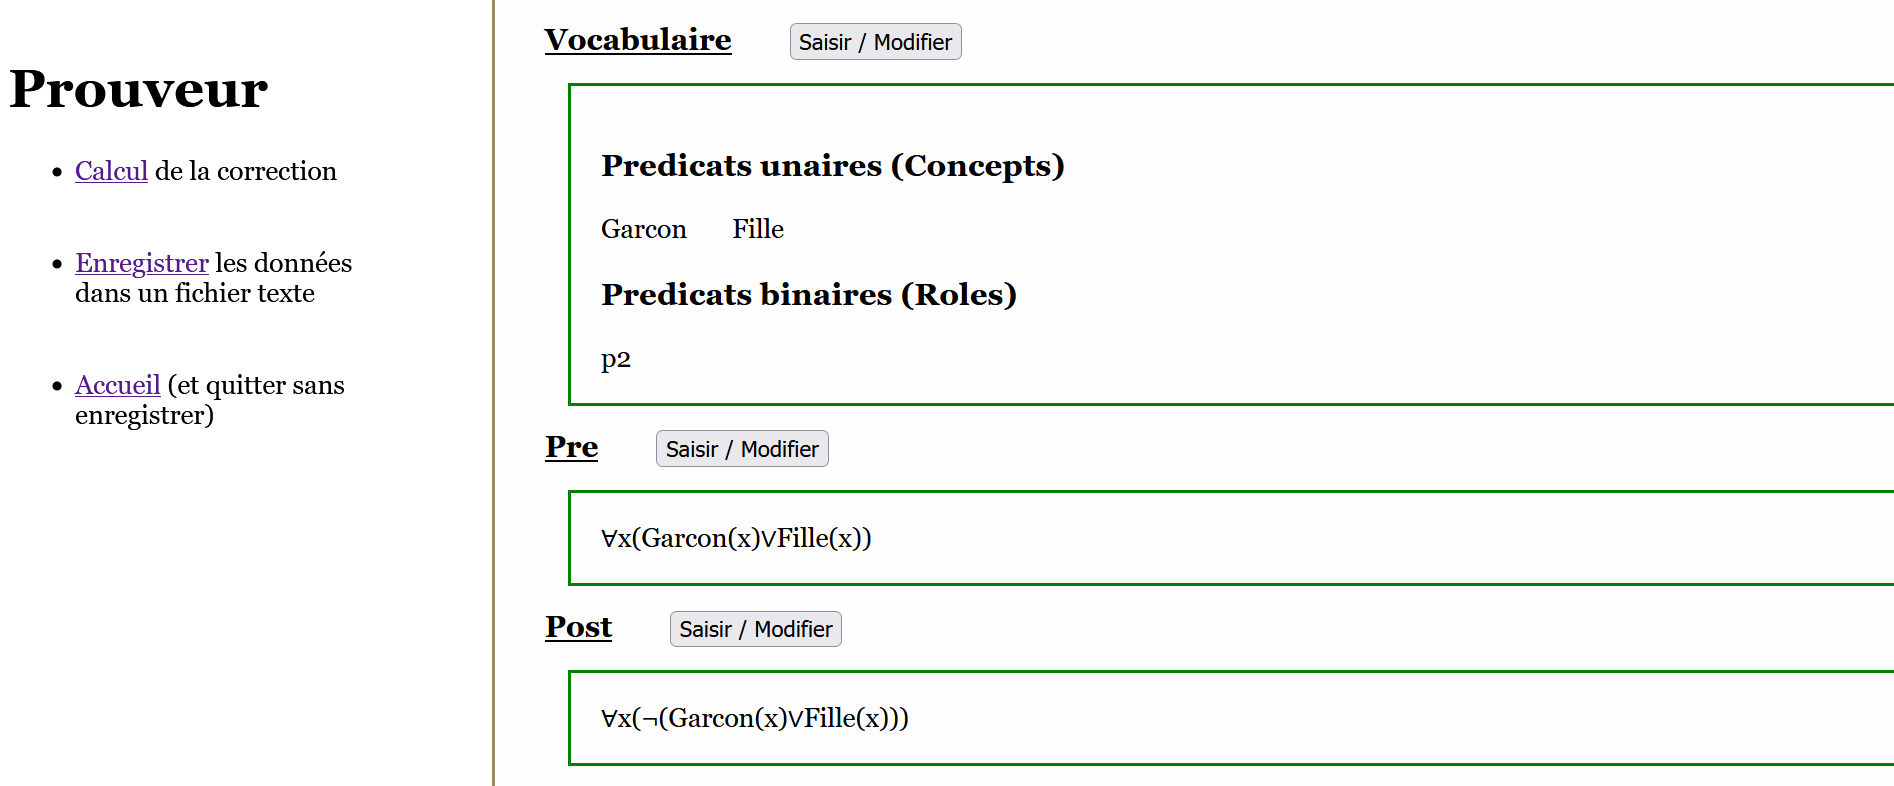
\includegraphics[width=0.6\textwidth]{screen5.png}
  \caption{Vue d'ensemble partie I}
  \label{fig:mon_image}
\end{figure}
\begin{figure}[htbp]
  \centering
  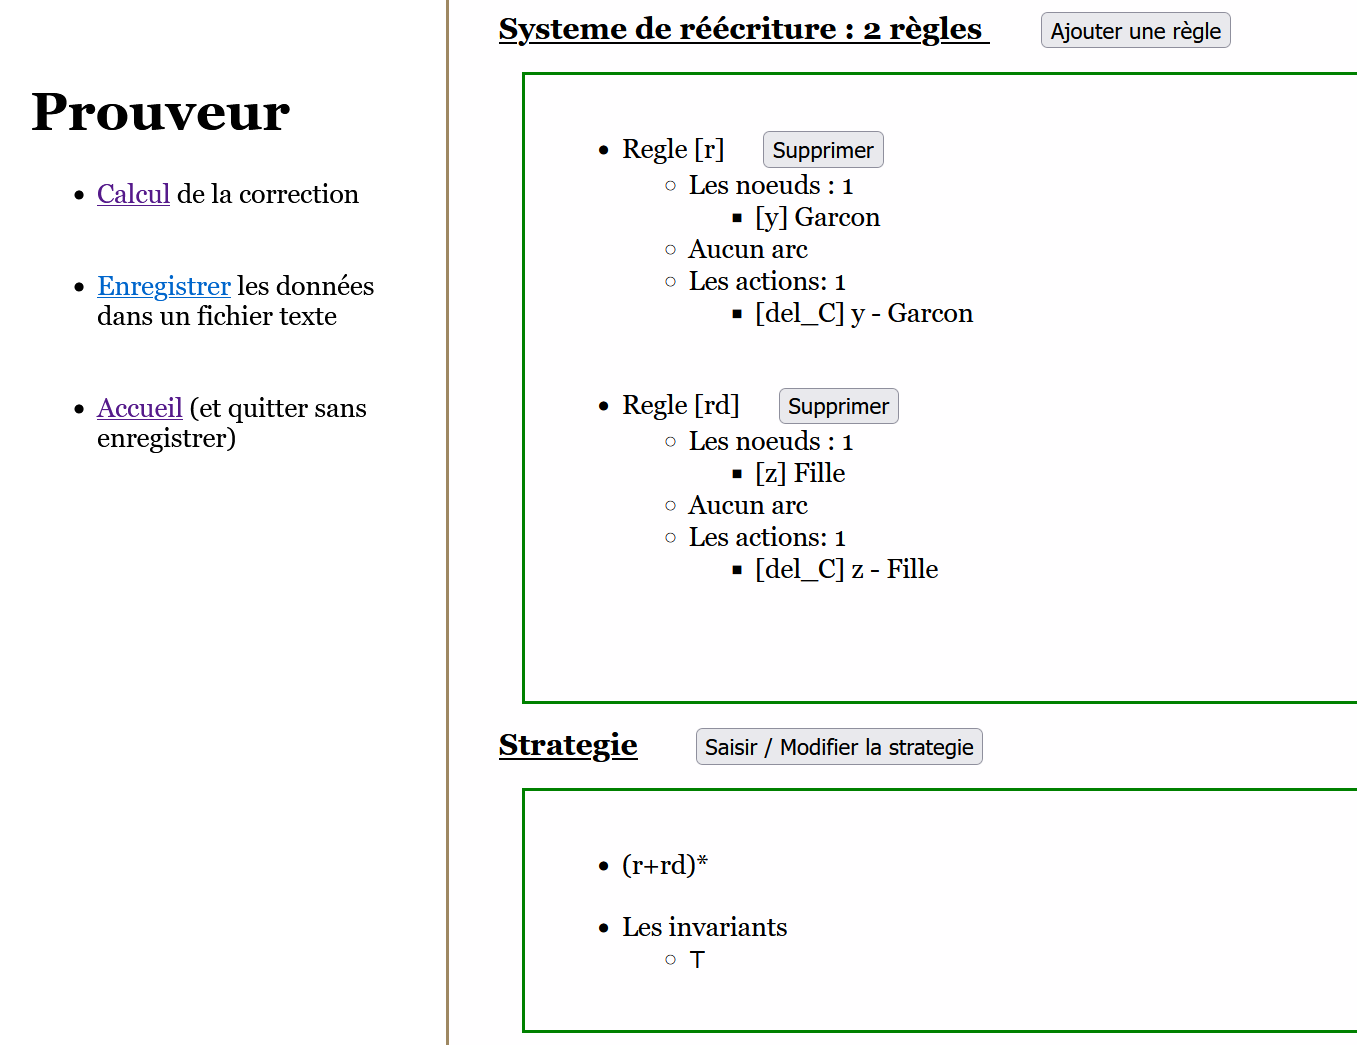
\includegraphics[width=0.6\textwidth]{screen6.png}
  \caption{Vue d'ensemble partie II}
  \label{fig:mon_image}
\end{figure}
\subsection{Saisie du vocabulaire}
La saisie du vocabulaire ou sa modification ouvre un formulaire dans lequel nous devons \textbf{ligne par ligne} indiquer les noms des concepts et des rôles.
\begin{figure}[htbp]
  \centering
  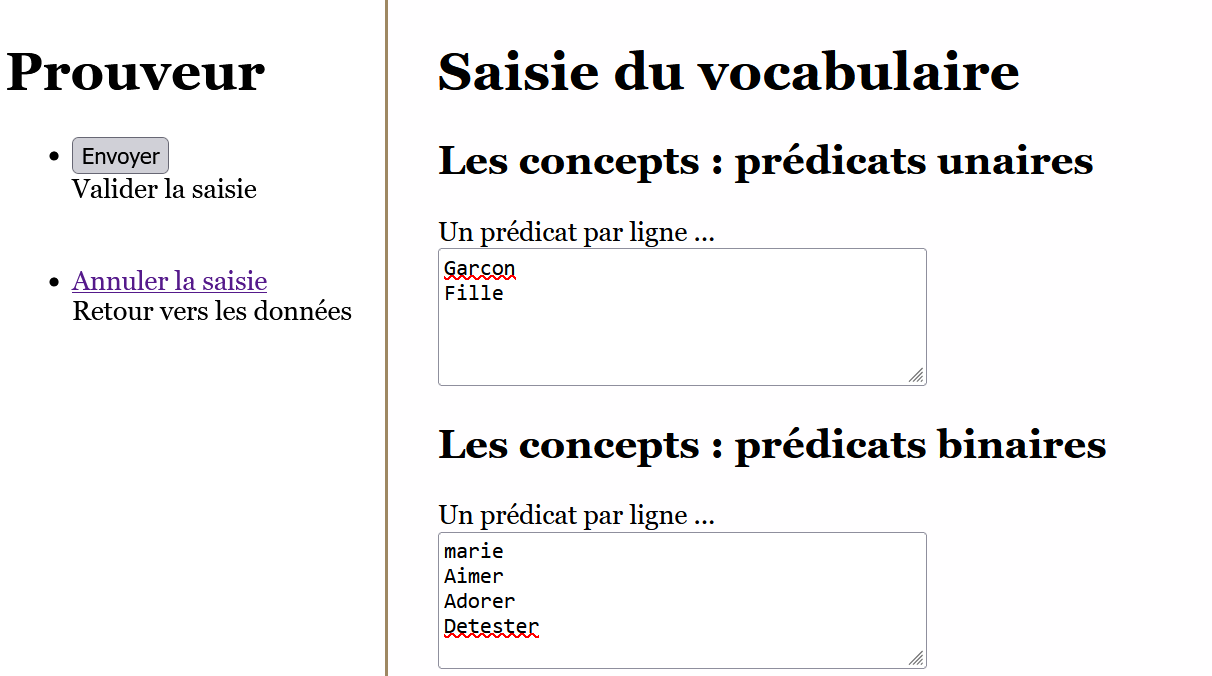
\includegraphics[width=0.6\textwidth]{vocab.png}
  \caption{Exemple d'une saisie de vocabulaire}
  \label{fig:mon_image}
\end{figure}
\subsection{Saisie des conditions (Pre et Post)}
\begin{figure}[htbp]
  \centering
  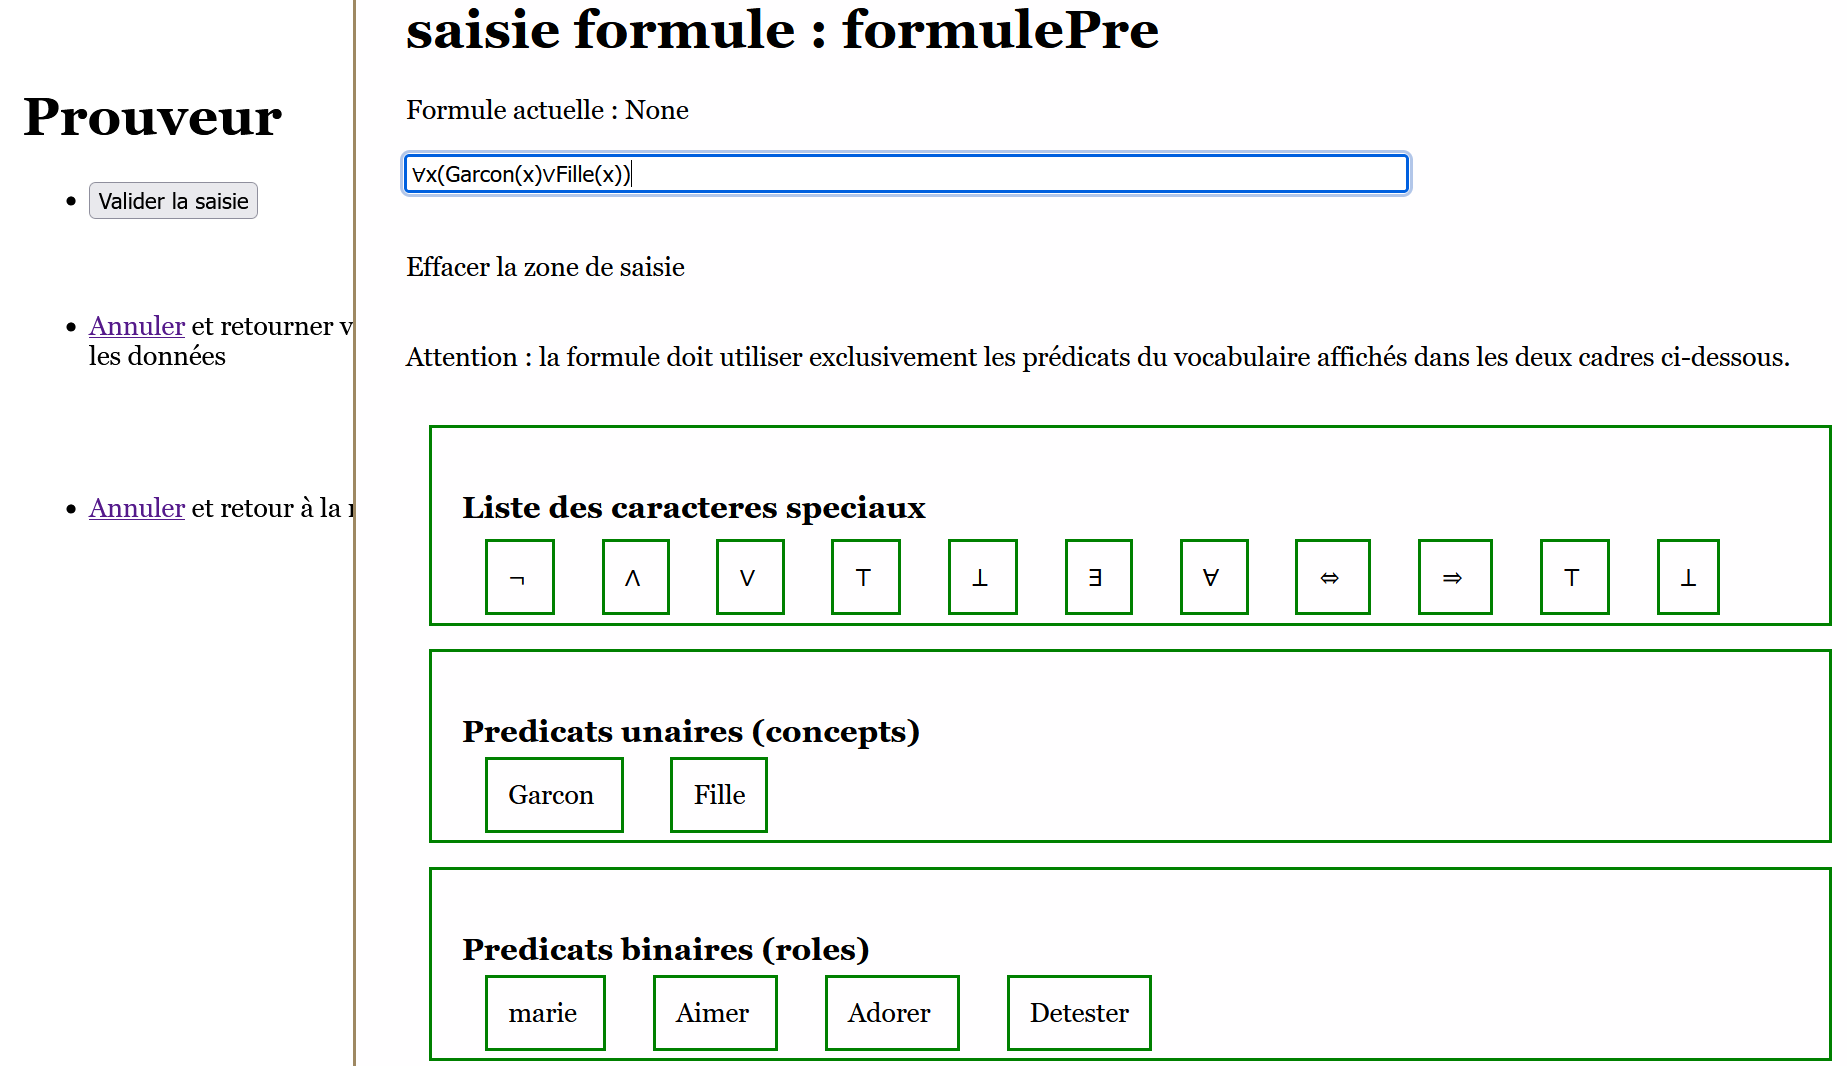
\includegraphics[width=0.6\textwidth]{screen7.png}
  \caption{Saisie des conditions (Pre et Post)}
  \label{fig:mon_image}
\end{figure}
Des boutons sont proposés pour faciliter l'écriture des caractères ascii. Attention: les "$\exists$" ainsi que les "$\forall$" doivent être entourés de parenthèses comme l'exemple ci-dessus. Les parenthèses des autres opérateurs peuvent être omises car le Lexer est souple -- mais il est tout de même conseillé de les mettre pour votre compréhension et pour éviter toute ambiguïté.
\subsection{Saisie d'une règle}
\subsubsection{Le lefthandside}
On code, un par un, les nœuds et les arcs \textbf{ligne par ligne} en suivant un format bien précis expliqué dans le formulaire. Si l'on souhaite qu'un nœud soit constant (qu'il ne soit pas appliqué à un pattern-matching), un tilde '$\sim$' doit être présent dans le nom du nœud. Ci-dessous, il y a un exemple d'une règle avec deux noeuds et un arc qui représente le fait qu'un homme appelé Gerome se marie avec une quelconque femme $x$ qu'il aime déjà. 
\begin{figure}[htbp]
  \centering
  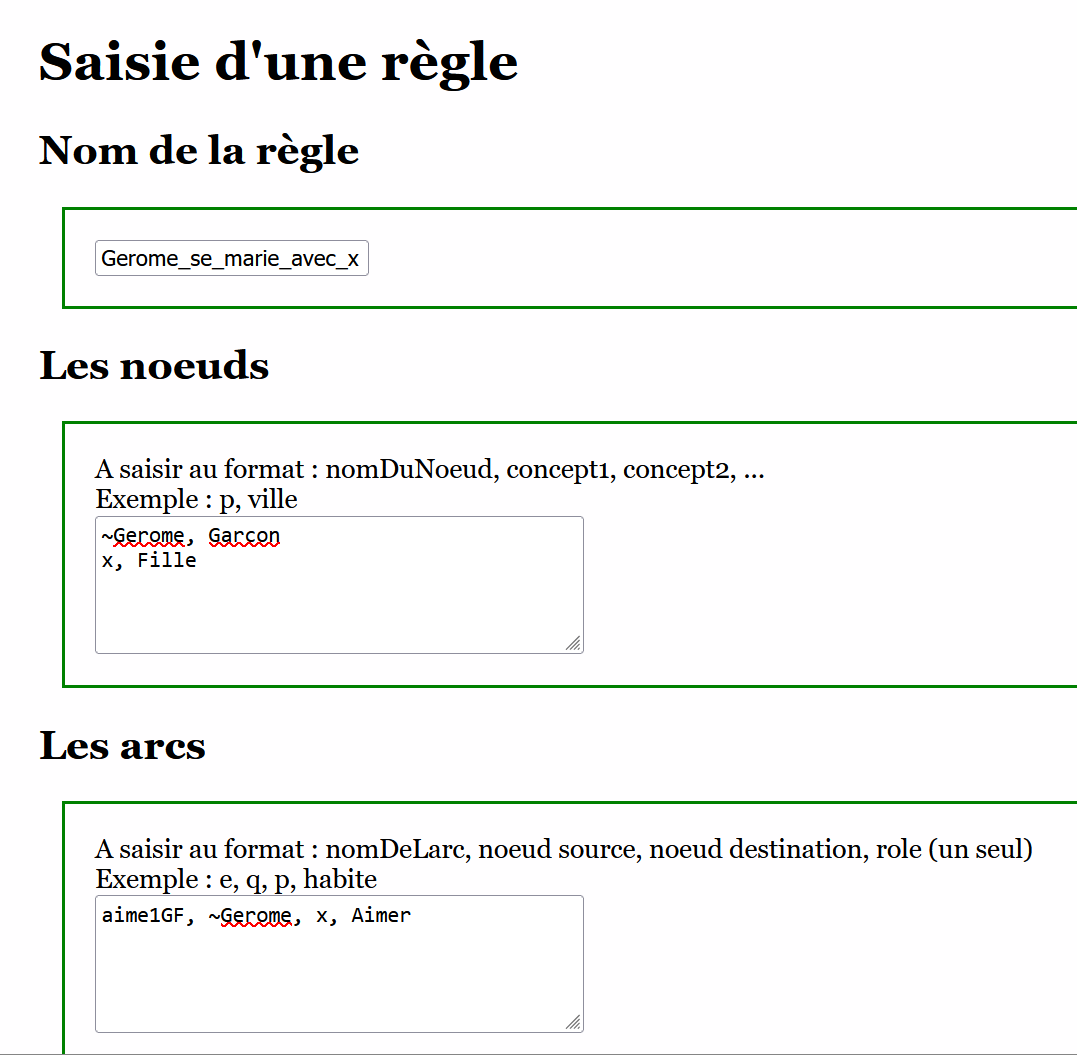
\includegraphics[width=0.6\textwidth]{screen8.png}
  \caption{Le lefthandside de l'exemple}
  \label{fig:mon_image}
\end{figure}
\subsubsection{Le righthandside}
Le rhs fonctionne de manière similaire. \textbf{Ligne par ligne}, on indique des actions élémentaires sous certains formats précis du formulaire. Cf. Figure 7 (ci-dessous)
\begin{figure}[htbp]
  \centering
  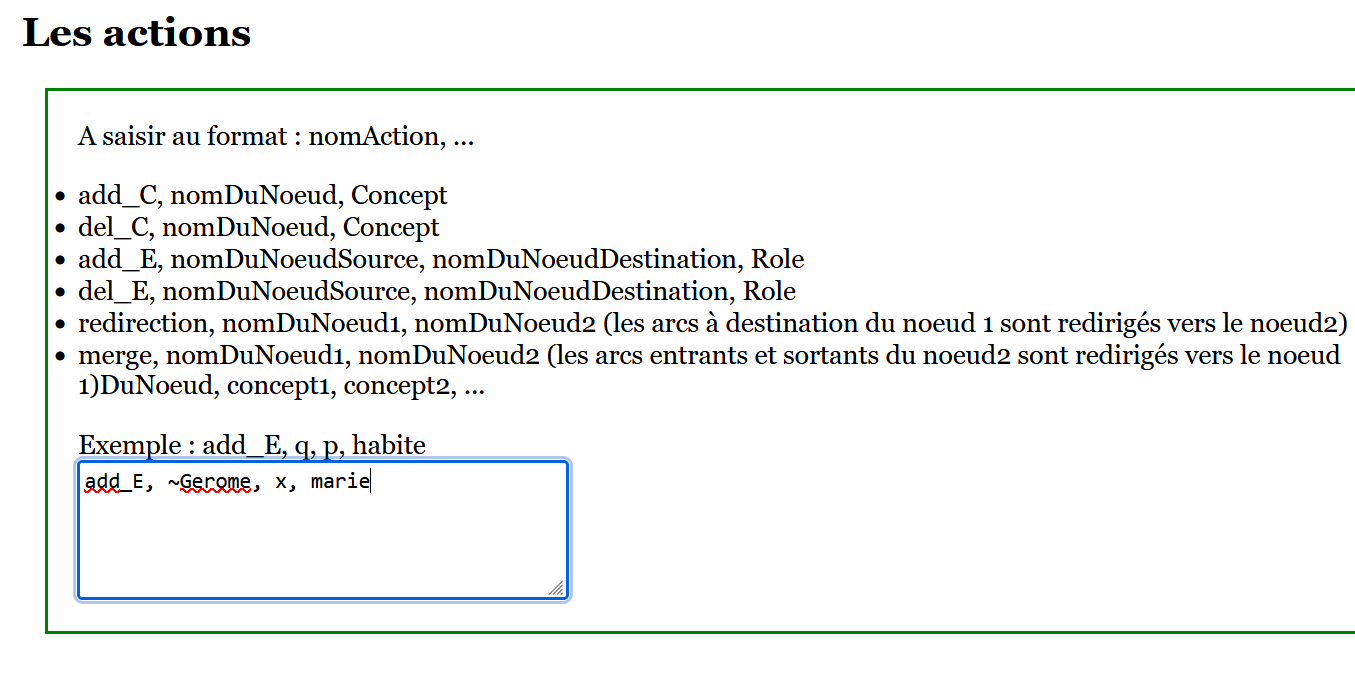
\includegraphics[width=0.6\textwidth]{screen9.png}
  \caption{Le righthandside de l'exemple}
  \label{fig:mon_image}
\end{figure}
\subsection{Correction}
\subsubsection{Formule}
Quand l'utilisateur a bien vérifié toutes les données de sa preuve, il clique sur "Calcul de correction". Il est alors dirigé vers une page qui contient entre autre la formule de correction.
\begin{figure}[htbp]
  \centering
  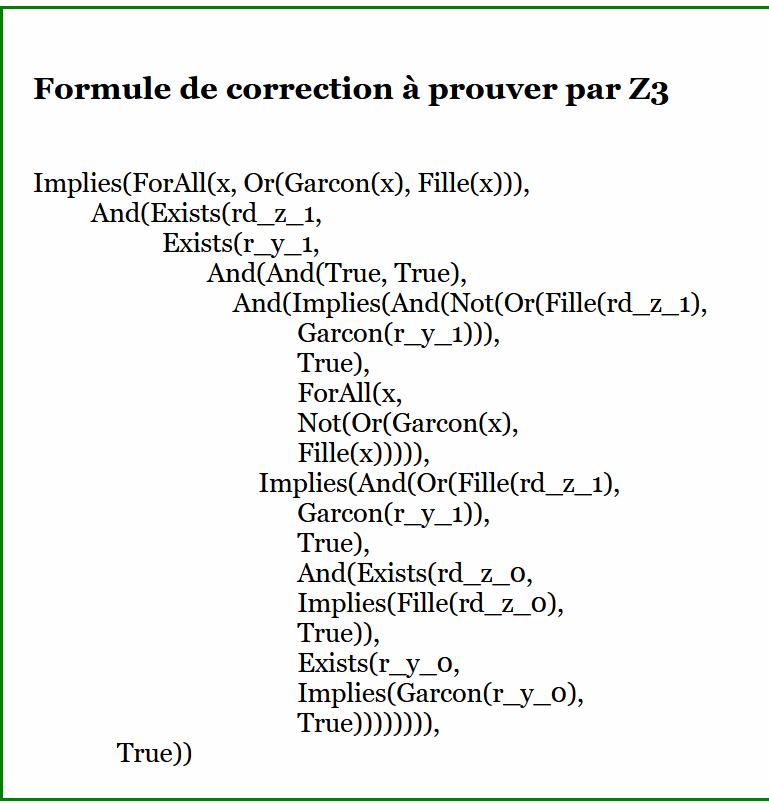
\includegraphics[width=0.6\textwidth]{screen111.png}
  \caption{Le righthandside de l'exemple}
  \label{fig:mon_image}
\end{figure}

Remarque: dans l'application des règles et des strategies, les noeuds des lhs, qui sont des variables, sont précédé par un  $\exists$ et renommés par "nomDeLeurRegle\_nomDuNoeud\_i". "i" étant le nombre de fois que la règle est appliqué.

\subsubsection{Réponse \& Modele brute}
Une réponse courte est aussi donnée à l'utilisateur pour dire si la preuve est valide ou non. Dans un cas où elle n'est pas valide, le modèle z3 (le contre exemple) est laissé pour les utilisateurs les plus agairis qui connaissent z3 et/ou qui sont dans la recherche.
\begin{figure}[htbp]
  \centering
  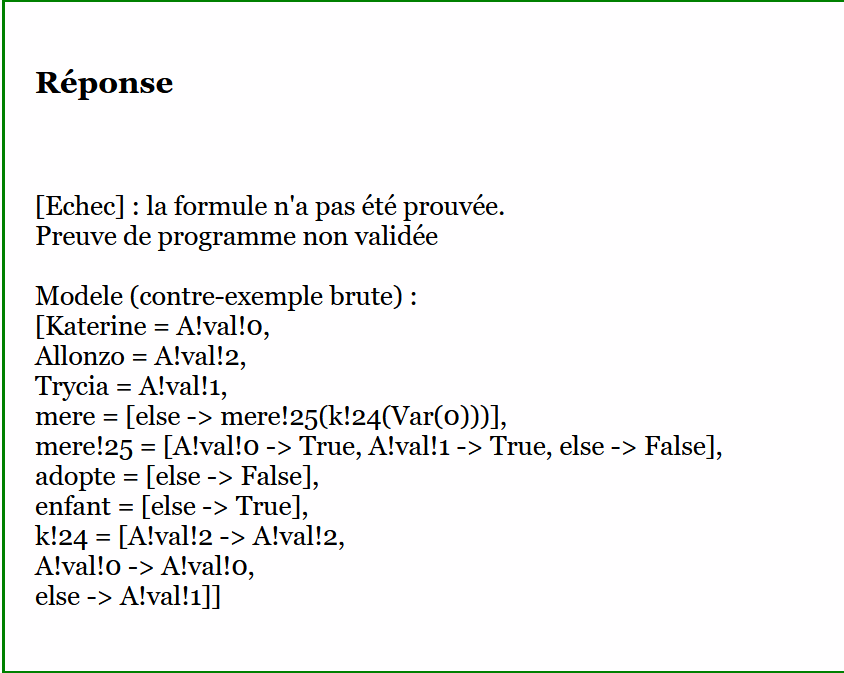
\includegraphics[width=0.6\textwidth]{sceen112.png}
  \caption{Reponse corte et modele brute}
  \label{fig:mon_image}
\end{figure}

\subsubsection{Contre-exemple}
Ces modèles brutes de z3 sont souvent incompréhensibles, ou du moins pas parlant. Le logiciel possède alors un affichage de contre-exemple. Pour chaque role ou concept, ça indique quels noeuds ou arcs les possèdent. Dans l'exemple, ci-dessous, Figure 10, Katerine, Allonzo ainsi que Trycia sont des noeuds du leftHandSide.

\begin{figure}[htbp]
  \centering
  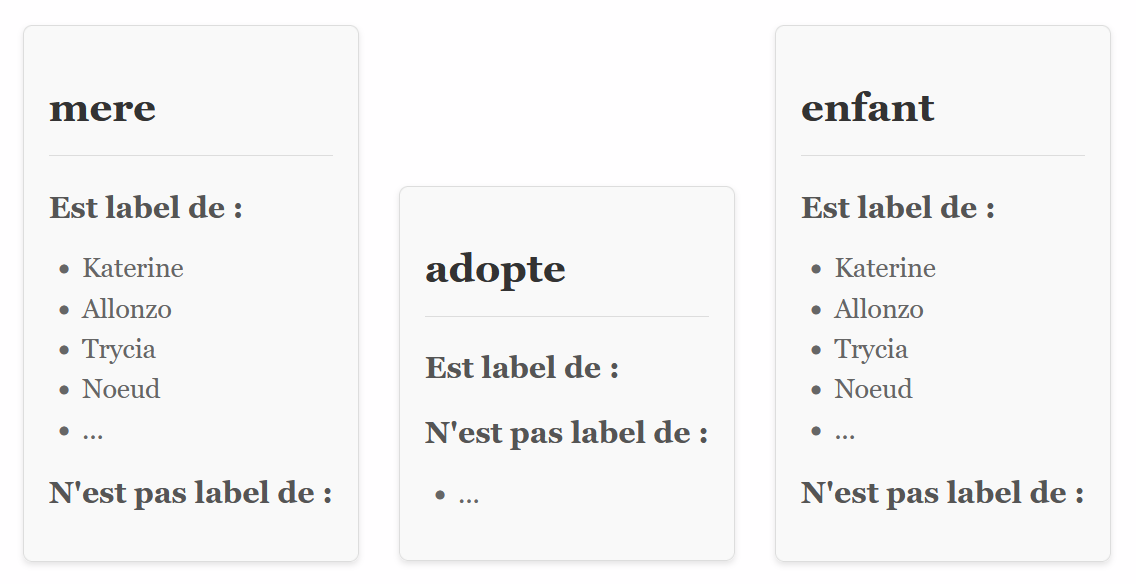
\includegraphics[width=0.6\textwidth]{screen113.png}
  \caption{Un exemple de contre-exemple}
  \label{fig:mon_image}
\end{figure}

Remarque :
\begin{itemize}
\item Le contre exemple est un graphe G (il peut en avoir plusieur) qui ne satisfait pas la preuve ;
\item les '...' signifient tous les autres noeuds (attributs possibles et imaginables) ;
\item les 'Noeud i' signifient des noeuds qu'on ne connait pas le nom, mais qui suffisent à montrer que la preuve est fausse pour le graphe G  ;
\item des éléments comme x!i ou elem!i peuvent apparaître dans les contre-exemples. Il s'agit de noeud souvent important dans le contre-exemple, mais parfois non. Ce sont des variables comme les Noeud i, cependant. 
\end{itemize}


\newpage
\section{Exemple d'utilisation}
Pour illustrer, nous allons nous arrêter à un exemple qui couvre beaucoup de cas d'utilisation. (Notez que plusieurs exemples sont laissés à l'utilisateur dans le dossier "Exemple". Ce dernier est invité à les générer dans l'application, dès l'écran d'accueil, en sélectionnant dans le menu "Lire un fichier".) \\

Soit $L$ un left-hand-side, dont le seul nœud est $k$. $k$ a comme unique concept $pred$. Soit $\alpha =  \texttt{del\_C(k, pred)} $ "on supprime le concept 'pred' d'un nœud". Soit $r = (L, \alpha)$.


\begin{figure}[htbp]
  \centering
  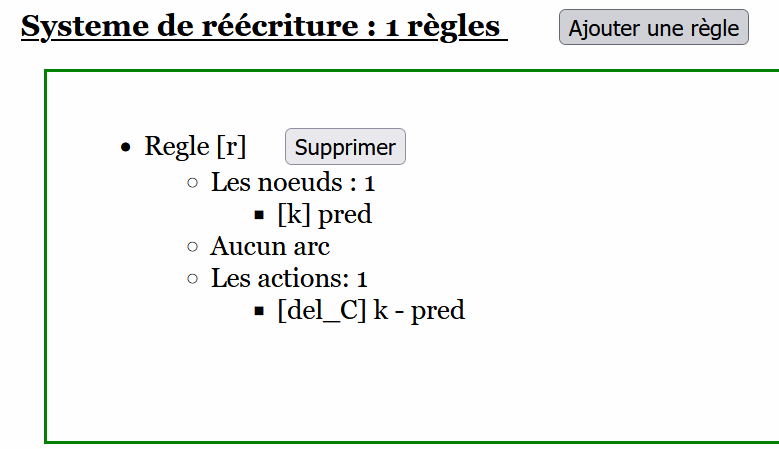
\includegraphics[width=0.6\textwidth]{screen1.png}
  \caption{La règle r}
  \label{fig:mon_image}
\end{figure}

Et on veut observer : 
\begin{enumerate}
\item $\{pred(x)\}r\{\lnot pred(x)\}$
\item $\{\forall x, pred(x)\}r\{\forall x, \lnot pred(x)\}$
 \item $\{\forall x, pred(x)\}r\{\exists x, \lnot pred(x)\}$
\item $\{\forall x, pred(x)\}r^{*}_{\{\top\}}\{\forall x, \lnot pred(x)\}$
\end{enumerate}
En d'autres termes, nous voulons montrer qu'à la fin, la règle supprime bien le concept du (des) nœud(s).\\ 
Il est très important de comprendre que le $1.$ va être prouvé par le logiciel. Quand l'utilisateur ne précise pas la quantification de la variable $x$, ça reviendrait à dire que $x$ est une variable libre. On peut aussi dire que $1.$ est équivalent à $\{\exists x, pred(x)\}r\{\exists x, \lnot pred(x)\}$. Ce qui est tout le temps vrai, car s'il existe au moins un nœud $x$ et qu'on applique $r$, à la fin il existera forcément un nœud $x'$ qui n'aura pas le concept $pred$.

\begin{figure}[htbp]
  \centering
  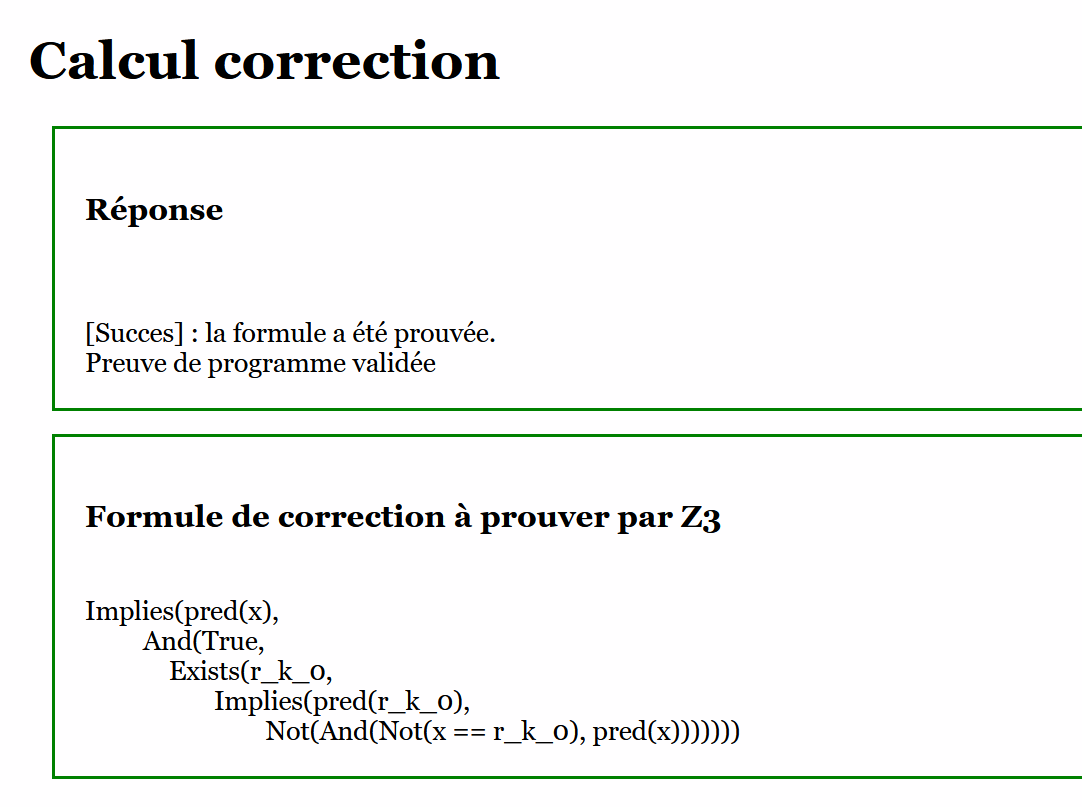
\includegraphics[width=0.6\textwidth]{screen2.png}
  \caption{Réponse de la correction du $1.$}
  \label{fig:mon_image}
\end{figure}


Par contre, le $2.$ est faux. Et l'application évidemment ne le prouve pas. Car, si on applique une fois \textbf{et une seule fois} $r$ aux graphes qui ont plusieurs nœuds (ayant le concept $pred$), on applique $r$ à un seul nœud. Donc, la postcondition $\{\forall x, \lnot pred(x)\}$ n'est pas respectée. L'application donne, d'ailleurs, un contre-exemple où il y a plein de nœuds qui ont le concept $pred$, représenté par '...' :

\begin{figure}[htbp]
  \centering
  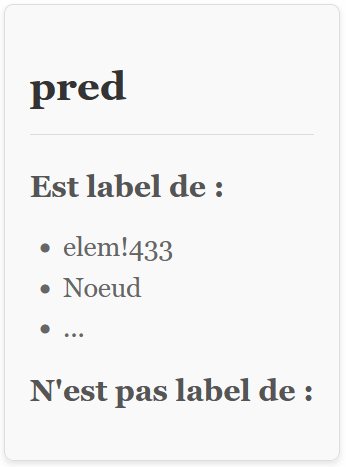
\includegraphics[width=0.3\textwidth]{screen114.png}
  \caption{Contre-Exemple du $2.$}
  \label{fig:mon_image}
\end{figure}

Le $3.$ est cependant prouvé car, à la fin, il y a bien un seul nœud qui a été changé.\\

Enfin, le $4.$ a été prouvé. En effet, dans ce cas, on applique $r$ tant que c'est possible, c'est-à-dire sur tous les nœuds. Ce qui explique pourquoi il n'y a plus aucun nœud qui a le concept $pred$. Voici la réponse du $4.$ :
\begin{figure}[htbp]
  \centering
  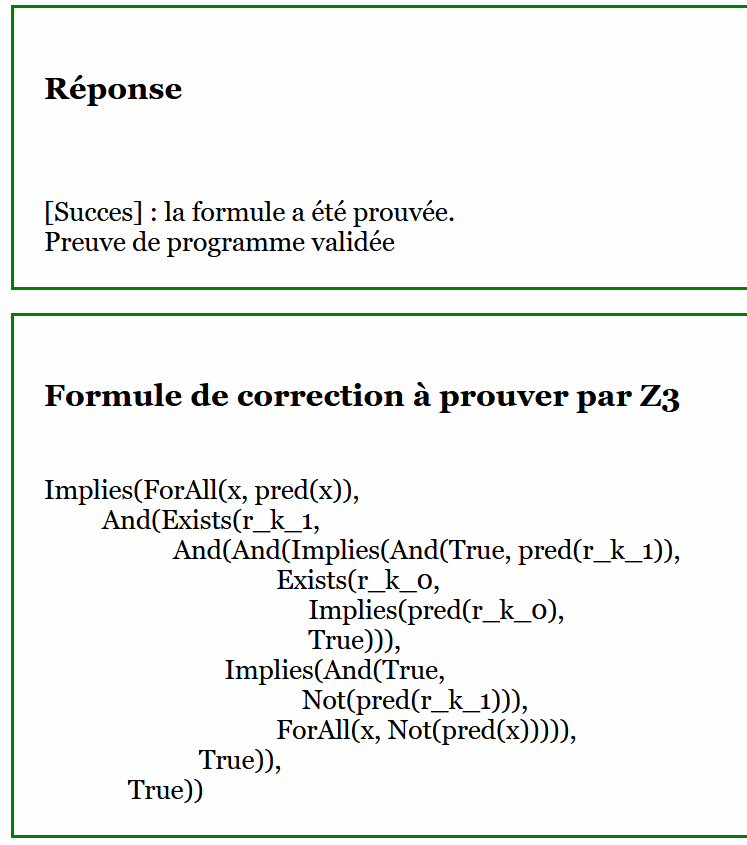
\includegraphics[width=0.6\textwidth]{screen3.png}
  \caption{Réponse de la correction du $4.$}
  \label{fig:mon_image}
\end{figure}
\end{document}
